% Este arquivo é uma adaptação do modelo LaTeX disponibilizado pelo UTUG (http://www.inf.ufrgs.br/utug/)
% Autor: Prof. Dr. Adriel M. Ziesemer Jr - IFRS Canoas
% O original encontra-se disponível em: https://sites.google.com/site/profadrielziesemer/home/modelolatexdetccparaoifrs
%
% Dica: Utilize o www.sharelatex.com para editar este documento. Utilize a opcão: Upload Zipped Project

\documentclass[openright]{ifrs} % utilize openright para iniciar capítulos no anverso
\usepackage[T1]{fontenc}        % pacote para conj. de caracteres correto
\usepackage[utf8]{inputenc}     % pacote para acentuaçao
\usepackage{graphicx}           % pacote para importar figuras
\usepackage{times}              % pacote para usar fonte Adobe Times
\usepackage{listings}
\usepackage{multirow}           % pacote para agrupar células em tabelas
\usepackage{scalefnt}           % pacote para redimensionar fontes em tabelas
\usepackage{amsmath}
\usepackage{rotating}           % pacote para rotacionar figuras
\usepackage{url}                % pacote para aceitar URLs (no .bib)
\usepackage{dirtytalk}          % pacote para aspas com comando \say{}

\usepackage{longtable}
\usepackage{cellspace}
\bibliographystyle{abnt}
\usepackage{array, tabularx, caption, boldline}
\usepackage{graphicx}
% ensine o latex a separar em sílabas as palavras que eventualmente ele não souber
\hyphenation{en-si-na-men-tos a-gra-de-ci-men-to de-se-nha-dos}

\author{Berwaldt de Oliveira}{Augusto}
%\author{Aluno2}{Nome do}

% edite o definicoes.sty se precisar alterar o nome do curso

\title{FERRAMENTA PARA AUXILIAR NO DIAGNÓSTICO DE DOENÇAS DE PELE}

\advisor[Prof.~Dr.]{Pinto}{Rafael Coimbra}


\location{Canoas}{RS}
%\date{julho}{2012} % se nao especificada, é utilizada a data atual

% palavras-chave (começar com letra maiúscula)
\keyword{Diagnóstico por Imagens}
\keyword{Pele}
\keyword{Doenças}
\keyword{Inteligência artificial}



% inicio do documento
\begin{document}

% folha de rosto
\maketitle

% dedicatoria (opcional)
\clearpage
\begin{flushright}
\mbox{}\vfill
{\sffamily\itshape
Dedico este trabalho à minha família.}
\end{flushright}

% agradecimentos (opcional)
\chapter*{Agradecimentos}
Agradeço  à minha família por ter formado minhas bases, aos professores
por me ajudarem a crescer, mas agradeço principalmente ao meu orientador  por 
ter aceito e me ajudado no desenvolvimento do meu projeto.
% resumo
\begin{abstract}
Tratamentos para doenças de pele são mais eficientes quando  as mesmas são detectadas precocemente,
especialmente antes que se espalhem para outros órgãos.
A análise dessas lesões geralmente é realizada através de exames de dermatoscopia, 
um exame não invasivo que utiliza um equipamento óptico para auxiliar na análise das estruturas que caracterizam as lesões.
Porém, a realização dessa análise geralmente é feita por um especialista, o que dificulta o acesso a esse exame.
Dessa forma, o uso de sistemas computacionais para auxiliar no diagnóstico pode facilitar o acesso a esse tipo de exame, tendo em vista que, com a ajuda do sistema, pacientes sem conhecimento  poderão ter uma análise das lesões de forma mais rápida. O aumento da quantidade de sistemas web adaptáveis a dispositivos móveis e a facilidade de acesso a internet resultou na utilização cada vez maior de  sistemas inteligentes para facilitar a vida das pessoas. A conveniência do uso de um sistema para a classificação de lesões de pele pode melhorar o acesso ao exame de dermatoscopia,
assim como aumentar a probabilidade de detecção precoce de alguma doença de pele.
Deste modo, este trabalho apresenta o desenvolvimento de um sistema de classificação de imagens dermatoscópicas para plataforma web.
 \end{abstract}

% resumo na outra lingua (opcional)
\begin{englishabstract}
{Skin disease diagnosing helper tool}
{Image diagnosis. Skin. Diseases. Artificial Intelligence}

Skin disease treatments are more efficient when those diseases are diagnosed early, especially before they spread to other organs.
These lesions analysis are generally made through dermatoscopy exams, a non-invasive exam that utilizes an optical equipment to aid on the analysis of structures that characterize the lesions. However, the analysis realization is generally made by an especialist, and that  difficults the access to this exam. This way, the use of computational systems to aid on diagnosis can make it easier to access this kind of exam, considering that, with the system help, pacients without knowledge can have a lesion analysis in a quicker way. The increase on the quantity of web systems adaptable to mobile devices and the easy internet access  resulted on a increasingly use of smart systems to ease people lifes. The convenience of using a system for skin lesions classification may improve the access to dermatoscopy exams, as well as raise the early detection probability of a skin disease.
This way, this work presents the development of a dermatoscopy image classification system for the web platform.
\end{englishabstract}

% lista de abreviaturas e siglas
\begin{listofabbrv}{SPMD}
        \item[API]Interface de Programação de Aplicativos (\textit{Application Programming Interface})
        \item[CSS] Folhas de estilo em cascata (\textit{Cascading Style Sheets})
        \item[ER] Entidade Relacionamento
        \item[HTML]Linguagem de Marcação de Hipertexto
        (\textit{HyperText Markup Language})
        \item[HTTP] Protocolo de Transferência de Hipertexto
        (\textit{Hypertext Transfer Protocol})
        \item[IBM] Empresa da área de TI (\textit{International Business Machines})
        \item[IDE] Ambiente de desenvolvimento integrado (\textit{Integrated Development Environment }) 
        \item[JS] JavaScript
        \item[JSON] Notação de Objetos 
        (\textit{JavaScript Object Notation})
         \item[MVC] Modelo-visão-controlador
        (\textit{Model-view-controllern})
        
        \item[SBC] Sociedade Brasileira de Dermatologia
        \item[SGBD] Sistema de gerenciamento de banco de dados
        \item[SQL] Linguagem de Consulta Estruturada (\textit{Structured Query Language})
        \item[TADS] Curso Superior de Tecnologia em Análise e Desenvolvimento de Sistemas
        \item[UML] Linguagem de Modelagem Unificada (\textit{Unified Modeling Language})
        
        
\end{listofabbrv}

% lista de figuras
\listoffigures

% lista de tabelas
\listoftables

% lista de símbolos (opcional)
%\begin{listofsymbols}{$\alpha\beta\pi\omega$}
%       \item[$\sum{\frac{a}{b}}$] Somatório do produtório
%       \item[$\alpha\beta\pi\omega$] Fator de inconstância do resultado
%\end{listofsymbols}

% sumário
\tableofcontents

\chapter{Introdução}
O processamento de imagens teve sua origem por volta da década de 1920, com melhoramento de imagens digitalizadas para jornais enviadas por meio de cabo submarino de Londres para Nova Iorque em 1920. Entretanto, a partir da década de 1960, quando imagens da Lua foram processadas com o intuito de remover distorções, estas técnicas serviram de base para métodos aprimorados de realce e restauração de imagens de outros programas. Com isso, esta área começou a ter o seu potencial reconhecido \cite{Gozalez}. Com o avanço dessa área da computação, têm surgido mais aplicações englobando diversas áreas como climatologia, medicina, eletrônica digital.

O trabalho aborda a área da Medicina, na qual cada vez mais tem se realizado pesquisas e desenvolvimento de soluções para a tomada de decisões médicas com o auxilio do processamento de imagens. A tomada de decisão é um procedimento comum durante a atividade de um médico. Uma dessas atividades é a interpretação e avaliação dos resultados de exames laboratoriais. Entre as doenças analisadas pelos médicos estão as doenças dermatológicas. A pele é o maior órgão do corpo humano e também o afetado pelo maior número de doenças. As doenças de pele mais comuns são foliculite, rosácea, melasma, alergia, psoríase, fungos e até mesmo o câncer \cite{SBC}. A partir disso, este trabalho busca desenvolver um sistema que ajude pacientes a identificar precocemente este tipo de doença, e com isso aumentar as chances de tratamento e melhorar a qualidade de vida dos pacientes.

Com o objetivo de auxiliar no processo de diagnóstico de doenças de pele o projeto visa o desenvolvimento de um sistema computacional baseado em conceitos de inteligência artificial e processamento de imagens digitais. Busca-se com este sistema a detecção de possíveis padrões característicos de determinadas doenças, como psoríase e melanoma, e uma vez detectados tais padrões, pode se  analisar imagens com as características das doenças. Os algoritmos de processamento de imagens digitais visam melhorar a qualidade das imagens ou destacar regiões de interesse.

As redes neurais artificiais têm sido frequentemente utilizadas sem problemas de reconhecimento de padrões e classificação devido à sua capacidade de aprender por meio de exemplos. Essa capacidade de aprender advém do processo de aprendizado, onde um conjunto de treinamento é interativamente apresentado à rede, a qual, a partir do algoritmo de aprendizado, constrói uma representação interna do problema,realizando um mapeamento, geralmente não-linear, entre as entradas e suas respectivas saídas \cite{haykin2001redes}.

Alguns sistemas inteligentes utilizam imagens previamente processadas na
formação de seu conjunto de treinamento,
permitindo a identificação de padrões que caracterizem grupos de interesse.
Devido ao impacto deste conjunto na capacidade de aprendizado e generalização da rede neural, deve-se buscar um aumento na qualidade das imagens antes de iniciar o 
treinamento do sistema. \cite{haykin2001redes}.

A medicina beneficia-se muito com o desenvolvimento de técnicas computacionais responsáveis pela ampliação da capacidade e da qualidade dos diagnósticos de diversas doenças, através da análise de imagens digitais. Estes diagnósticos vêm apresentando resultados significativos e auxiliando vários profissionais da saúde. Dentre os trabalhos desenvolvidos que unem computação e medicina, o diagnóstico de doenças por imagem oferece um grande recurso para a área médica.

O objetivo deste trabalho é descrever o desenvolvimento de um sistema computacional de apoio ao diagnóstico de doenças de pele, que utiliza técnicas de inteligência artificial e processamento de imagens visando à melhoria da informação visual, permitindo posteriores análises, para identificar as possíveis doenças que podem vir a ser detectadas nas imagens. Será utilizado o sistema IBM Watson para englobar a maior parte do processo de classificação e aprendizado do sistema. IBM Watson é um sistema do tipo cognitivo que possibilita uma nova parceria entre pessoas e computadores.

O sistema IBM Watson possui um serviço de  reconhecimento visual de imagens, disponibilizado via API, onde é possível criar classificadores para treinar um determinado nicho de imagens. O sistema utiliza-se de algoritmos de aprendizagem profunda (Deep Learning), para realizar a classificação das imagens. Esse tipo de algoritmo faz parte do subcampo de aprendizado de máquina.


\section{Motivação}
As tecnologias foram evoluindo possibilitando o desenvolvimento de sistemas computacionais que auxiliassem dermatologistas e profissionais da área da saúde na análise de lesões de pele. Os sistemas de visão computacional estão sendo cada vez mais utilizados como ferramentas de apoio para análise do melanoma. Esses sistemas geralmente utilizam imagens de lesões de pele para extrair as informações das lesões utilizando algoritmos médicos e classificam essas informações utilizando algoritmos de aprendizagem de máquina.

A difícil tarefa de analisar lesões dermatoscópicas para o diagnóstico do melanoma tem influenciado o desenvolvimento de novos métodos que auxiliem o ser humano na realização dessa tarefa. Isso mostra que sistemas inteligentes que trabalham com imagens passam a ser de grande interesse e com um potencial enorme a ser explorado como ferramentas de apoio ao diagnóstico de doenças de pele.

O diagnóstico de doenças com sistemas inteligentes de aprendizado é uma ideia já explorada, mas ainda um campo pouco desenvolvido. Sistemas inteligentes são sistemas que tentam simular o pensamento humano e tentam de forma lógica resolver problemas que pessoas resolveriam no cotidiano. Uma das características de sistemas inteligentes é justamente a capacidade de aprender, de se adaptar a uma situação nova assim como um ser humano se adaptaria \cite{rezende2003sistemas}.
\section{Objetivos}
Os objetivos foram organizados em objetivo geral (Seção 1.2.1) e específicos (Seção 1.2.2).
\subsection{Objetivo Geral}
Desenvolver um sistema web para auxiliar na prevenção e diagnóstico precoce de doença de pele, por meio de análise de imagens.
\subsection{Objetivos Específicos}
\begin{itemize}
 \item Estudar propostas existentes.
 \item Levantar os requisitos do sistema a ser desenvolvido.
 \item Implementar um sistema que solucione o problema apresentado sem custos para o usuário.
 \item Desenvolver Testes Funcionais.
 \item Escrever a documentação completa do sistema.
\end{itemize}

\section{Organização do Texto}
O documento está dividido em 7 capítulos. No primeiro capítulo é apresentada a ideia principal do projeto, a problemática principal, a motivação para a realização do trabalho, assim como os objetivos gerais e específicos. Há o capítulo que
explica os materiais e métodos utilizados para realização do trabalho. Os capítulos seguintes, contém os trabalhos relacionados, o referencial teórico e o levantamento de requisitos.
No capítulo 6 serão apresentadas as telas e principais funcionalidades do Skin System, seguido da apresentação dos resultados dos testes realizados com  a ferramenta e a conclusões do trabalho.
\chapter{METODOLOGIA}
A primeira etapa do projeto é constituída de pesquisa e coleta de dados para criação de referencial teórico e melhor definição dos objetivos da pesquisa. Foi realizado uma pesquisa do tipo acadêmica por meio de livros e pesquisa feita na web. Foi desenvolvido um protótipo que pode ser executado em ambiente Web. Os códigos foram desenvolvidos e testados na IDE Intellij que fornece um ambiente integrado de desenvolvimento. A linguagem definida foi Python, que é disponibilizada gratuitamente.

A segunda etapa foi a elaboração dos diagramas do sistema. Os diagramas do sistema seguiram o padrão de modelagem UML que é uma linguagem de modelagem de digramas universal  (GUEDES, 2009) . Foram desenvolvidos os diagramas de classe, diagrama de atividades, diagrama de sequência, diagrama ER. No desenvolvimento dos diagramas foi utilizado a ferramenta Astah \footnote{http://astah.net/editions/community}, que disponibiliza uma versão gratuita para estudantes.

A metodologia de desenvolvimento do sistema foi a metodologia cascata. O modelo cascata ou modelo waterfall,também é chamado de modelo tradicional de desenvolvimento de software. Ele organiza os projetos de software em quatro grandes fases realizadas sequencialmente: análise, projeto, codificação e testes, sendo que uma fase só inicia quando a anterior estiver completa. Ainda hoje este modelo de desenvolvimento é o mais conhecido e amplamente utilizado \cite{pressman2016engenharia}. Primeiramente houve o levantamento de todos os requisitos funcionais e não funcionais do sistema, para depois começar o desenvolvimento do sistema seguindo as quatro fases do modelo cascata. Ele deve seguir o que foi levantado pela análise dos requisitos. Nesse modelo de desenvolvimento os testes unitários serão realizados logo após a conclusão da ultima entrega da etapa de desenvolvimento.

Para realização dos testes foi utilizado a técnica de \textit{data augmentation} \footnote{O aumento de imagem cria artificialmente imagens de treinamento 
através de diferentes formas de processamento ou combinação 
de processamento múltiplo, como rotação aleatória, escalas diferentes entre outras funções. }, 
que realiza  modificações em cada imagem aplicando mudanças de escala, translação e rotação. Com isso podemos gerar mais imagens para ampliar a base de treinamento do classificador
que foi composta de 50 imagens da doença de melanoma e mais 50 imagens da doença de psoríase, 
que foram  mineradas na \textit{web}, então foi aplicado o \textit{data augmentation} para aumentar a base de treinamento 
do classificador. As medidas que foram utilizadas para alteração da escala, translação e rotação foram
para a escala (0.5, 2), (-100, +100) para translação  e para rotação 
foram utilizados os graus de (90,  180, 270, 360). Como para cada imagem será aplicado a técnica, teremos
para cada imagem  teremos mais  16 imagens , como teremos 80 imagens, pois foram retiradas 10 de cadas doença,
para realizar o teste de classificação, teremos então uma base com  1280 imagens para treinamento
do classificador.


Para gerar os testes foi utilizado a mesma técnica de \textit{data augmentation},
com as 20 imagens retiradas das imagens que foram mineradas para gerar a base de treinamento do classificador,
com isso o teste tera 320 imagens, que não fazem parte 
da base de treinamento do classificador.
  


O protótipo inicial foi testado por métricas estatísticas, utilizando a matriz de confusão para calcular a medida de acurácia \cite{medicinabaseadaemevidencias}. Acurácia é definida como a capacidade do método de acertar o diagnóstico. Com isso se pode verificar a taxa de autenticidade do diagnóstico da doença de pele. Esta etapa de teste deverá ser concluída para a obtenção de resultados satisfatórios e para ter uma prevenção de possíveis erros que poderão ser encontrados na aplicação. O resultado final do software foi  distribuído na plataforma web para posteriormente ter integração com outros sistemas.


\chapter{Estado da Arte}
Nesse capítulo serão apresentados projetos relevantes que foram ou estão sendo desenvolvidos na área de estudo deste trabalho. As ferramentas presentes na internet com o público-alvo semelhante ao do Skin system, têm geralmente versões apenas para iphone, ou focadas nesse tipo de sistema.

\section{Ferramentas comerciais}

\subsection{SkinVision}
SkinVision é uma solução on-line que apoia os indivíduos na avaliação  e condições de pele para risco de câncer de pele. Ele fornece uma solução de conscientização e rastreamento para que os usuários possam monitorar facilmente suas lesões ao longo do tempo. O SkinVision oferece uma tecnologia única e cientificamente comprovada para detectar sinais iniciais e potenciais de crescimento de câncer de pele.O algoritmo foi desenvolvido e testado em cooperação com dermatologistas e verifica as irregularidades na cor, textura e forma da lesão. O aplicativo é um dispositivo de diagnóstico precoce que ajuda o paciente a visitar o seu médico preparado e a tempo \cite{SKINVISION}. Na figura 3.1 é apresentada a interface do aplicativo SkinVision, onde ele apresenta como é realizada a coleta das imagens.


\begin{figure}  [h]
    \caption{Interface de usuário do SkinVision}
    \centerline{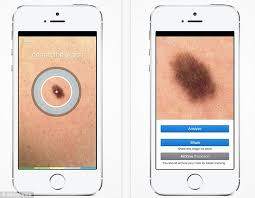
\includegraphics[width=20em]{figuras/download.jpg}}
    \centerline{Fonte: www.SkinVision.com}
\end{figure}


\vspace{2cm}

\subsection{Lūbax}
o sistema Lūbax é um sistema de diagnóstico de doenças de pele. Ele funciona de forma semelhante a um livro de texto, onde você pode encontrar uma imagem que se parece com seu problema de pele \cite{LUBAX}. Mas enquanto observar isso em um livro de texto levaria muito tempo, Lūbax faz isso em um instante. O algoritmo Lūbax funciona um pouco como uma busca de imagens do Google. O Lūbax atualmente só se encontra disponível para sistemas IOS, onde os usuários devem pagar para utilizar o sistema de diagnóstico. 

\begin{figure}  [h]
   \caption{ Interface de usuário do Lūbax}
    \centerline{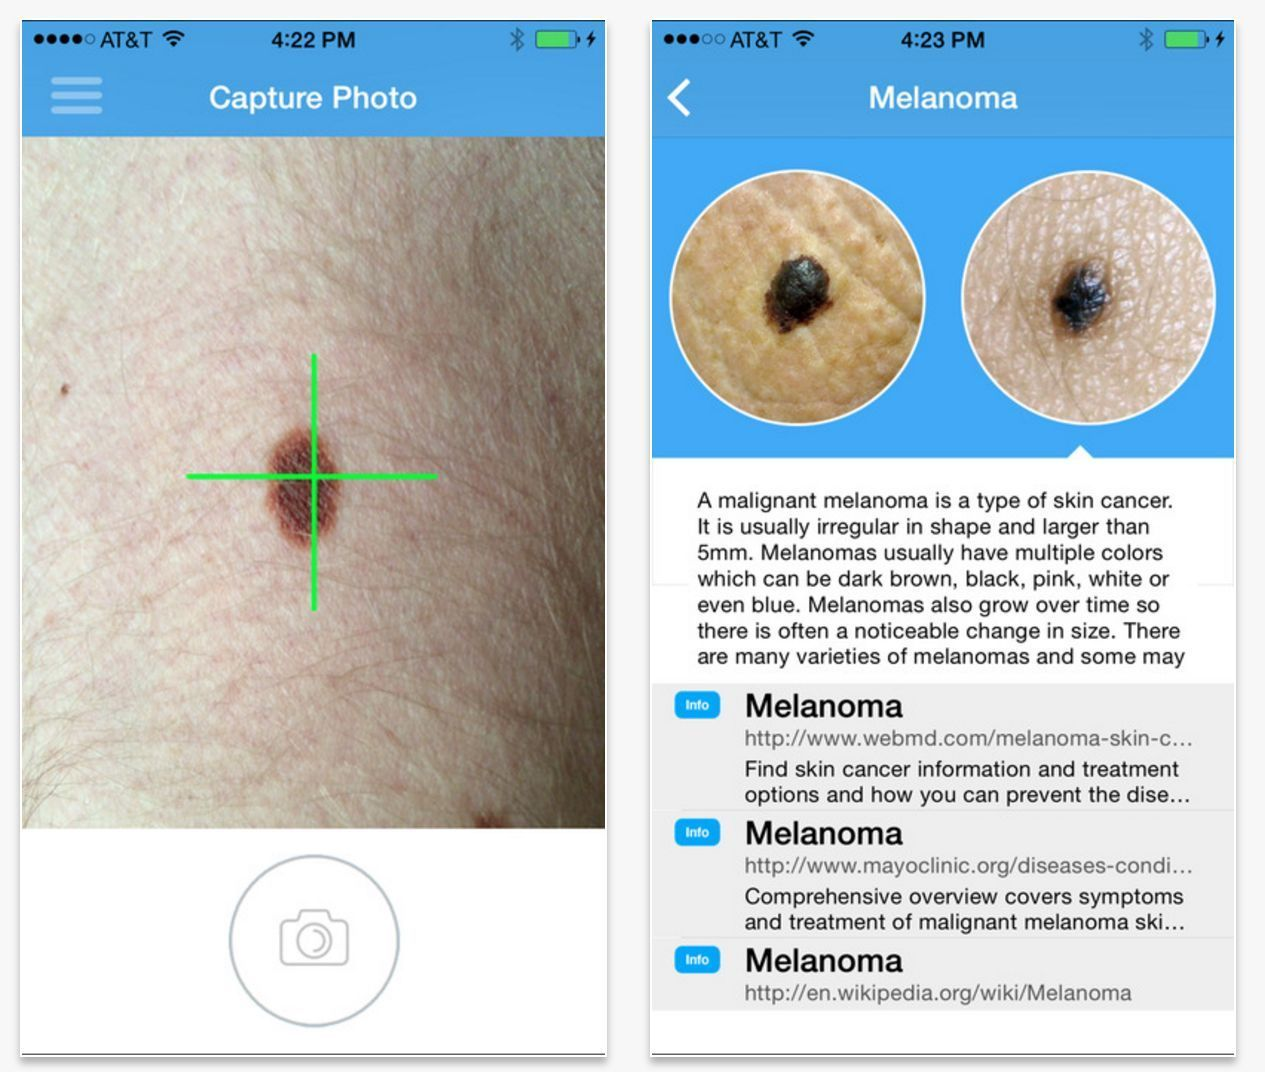
\includegraphics[width=20em]{figuras/lubax-100713688-orig.jpg}}
   
    \centerline{Fonte: www.lubax.com}
\end{figure}

\section{Trabalhos Científicos}

Entre os trabalhos científicos pesquisados estão as obras de Alencar  \citeyearpar{alencar2015desenvolvimento} e  Roberta Barbosa \citeyearpar{oliveira2012metodo}, ambos propuseram sistemas para auxiliar diagnóstico de lesões de pele por imagem. \par

Alencar propôs diretrizes para o desenvolvimento de uma aplicação \textit{mobile} com a intenção de auxiliar os diagnósticos de melanoma. Para isso, ele utilizou algoritmos  baseados em Redes Neurais Artificiais. Para realizar esse aplicativo foi utilizado algoritimo  
backpropagation, para treinar a rede neural baseada em Perceptrons de múltiplas camadas (\textit{Multilayer Perceptron}) MLP, que é considerada uma rede neural semelhante à rede perceptron. Também foi utilizado processamento de imagens para melhorar e extrair ruídos das imagens. Como resultados, o autor definiu a fundamentação teórica da pesquisa e desenvolveu um aplicativo \textit{mobile} para  auxiliar médicos e profissionais da saúde na análise do câncer de pele.



 Roberta Barbosa, em sua dissertação de mestrado, desenvolveu um
 método computacional capaz de auxiliar os médicos
dermatologistas no diagnóstico de lesões de pele por meio de imagens digitais. O método utilizou a regra ABCD (Assimetria, Borda, Cor e Diâmetro) e análise de textura, para identificar as
lesões. O projeto também usou o modelo Chan-Vese \cite{brown2012completely}, 
que é baseado na técnica de crescimento de região Mumford-Shah \cite{chan2001level}, para segmentar as imagens. Como conclusão o autor definiu que as informações obtidas pelo método podem ser disponibilizadas ao dermatologista com o objetivo de auxiliá-lo no diagnóstico das lesões de pele.


\section{Conclusão}

Neste capítulo foram apresentados trabalhos e sistemas existentes relacionados à temática e a proposta do Skin System. A grande diferença entre os sistemas comentados e o sistema proposto por esse projeto é a comercialização do sistema e sua distribuição em plataformas. Enquanto o sistema Lübax, por exemplo, cobra pela sua utilização e só está disponível para usuários da plataforma mobile IOS, o projeto da ferramenta de diagnóstico visa atender a todos dispositivos que possuam navegador. apresentando versão gratuita e futuramente em outra versão do sistema tera uma versão comercial com recursos adicionais. Outro diferencial é a utilização de API de um classificador ao invés de desenvolver um no proprio sistema, pois com isso pode-se ter um serviço distribuido e que já  é utilizado por outras companias.

\chapter{Referencial Teórico}
Neste capítulo serão abordados alguns conceitos importantes que estão presentes no desenvolvimento e metodologia do Skin System.


\section{Diagnóstico por Imagens}

As técnicas de diagnóstico por imagem começaram a se desenvolver apenas no final do século XIX e início do século XX, mas muito já foi aprimorado desde aquela época, quando o físico alemão Wilhelm Roentgen tentou discernir os ossos do corpo no primeiro raio-X da história. Atualmente, com todo o desenvolvimento tecnológico promovido, os exames de imagem já permitem a visualização de vasos sanguíneos e até a reconstrução em 3D de diversas estruturas biológicas.  No Brasil, o diagnóstico por imagem é uma especialidade médica conhecida como Radiologia e Diagnóstico por imagem que leva à formação de médicos radiologistas \cite{prando2015fundamentos}. 

O conceito de diagnóstico vem sendo aplicado em imagens mais simples como uma fotografia de uma lesão no corpo  através dessa imagem é possível a realização de uma análise, buscando características comuns a serem processadas. Para realizar essa análise de característica esse projeto utiliza-se das técnicas de processamento de imagem e visão computacional.


\section{Processamento de Imagem}
Processamento de imagens é um método para converter uma imagem em forma digital e executar algumas operações nela, para obter uma versão aprimorada da mesma ou extrair algumas informações relevantes dela. Esta área vem sendo objeto de crescente interesse por permitir a criação de grande número de aplicações que necessitem de extração de informação de imagens. \cite{marques1999processamento}.

O sistema visual humano tem uma grande capacidade de reconhecer padrões. No entanto, ele dificilmente é capaz de processar o enorme volume de dados presentes num estímulo visual. Por isso o principal objetivo do processamento de imagens é o de remover essas barreiras, inseparáveis ao sistema visual humano, facilitando a extração de informações a partir de imagens. Nesse contexto, o processamento digital deve ser encarado como uma fase preparatória, embora quase sempre obrigatória, da atividade de interpretação das representações gráficas, para que depois seja utilizado juntamente com as técnicas de visão computacional.

 
\section{Visão Computacional}

A visão computacional atua juntamente com o processamento de imagens, analisando conteúdo visual para obter resultados similares aos que o ser humano obtém através da visão. Visão computacional é a tecnologia e ciência responsável pela forma como o computador visualiza o meio à sua volta, extraindo informações significativas a partir de imagens capturadas por câmeras de vídeo, scanners entre outros aparelhos. Com essas informações se pode reconhecer, manipular, criar algoritmos capazes de interpretar o conteúdo e ainda pensar sobre os objetos que compõem uma imagem \cite{neves2012avanccos}.

O objetivo de um sistema de Visão Computacional é tomar decisões a partir da extração de informações do mundo real através de imagens. A partir dessa extração de informações se pode realizar a tomada de decisão a partir de indagações simples a respeito de parâmetros extraídos dos objetos ou de algoritmos mais complexos de Inteligência Artificial. Nesse trabalho esse conceito é essencial pois, como dito antes, o objetivo é extrair informações de imagens para uma análise e possível classificação de uma doença de pele. Para desenvolver esses conceitos de visão computacional, foi desenvolvido um aplicativo web adaptável a dispositivos móveis seguindo os princípios de desenvolvimento portátil.


\section{Desenvolvimento com Portabilidade}
Com a popularização da programação voltada a dispositivos móveis, surgiu o conceito de Design Responsivo. A responsividade permite uma melhor visualização para todos dispositivos. Segundo \citeauthor{zemel2015web}, o conceito de web design responsivo é  definido como qualquer design que acessado por qualquer dispositivo ou resoluções que respeita uma série de características técnicas bem específicas, será  bem apresentado em qualquer  dispositivo.

\section{Materialize}

Para utilizar um design responsivo e adaptável será utilizado o \textit{framework}\footnote{http://www.dsc.ufcg.edu.br/~jacques/cursos/map/html/frame/oque.htm} Materialize\footnote{http://materializecss.com}, para desenvolvimento do layout desse trabalho.O Materialize é gratuito e possui uma vasta biblioteca de funcionalidades para serem implementadas em web sites.

 Ao baixar o pacote do Materialize, há arquivos escritos em Javascript, CSS e até mesmo fontes de letras. O arquivo CSS tem um vasto conteúdo pronto para utilização e formatação automática a ser inserida nas tags de HTML contidas nos arquivos principais de um \textit{web site}. Dentro do próprio site do Materialize há guias de conteúdo para criação de formulários, menus de navegação, botões, tabelas e muitas outras funcionalidades típicas de desenvolvimento web com um padrão moderno, simplificando assim a implementação de web sites responsivos.

\section{Cliente}

\subsection{HTML e CSS}
O sistema terá suas interfaces visuais desenvolvidas em HTML que é a linguagem principal de quase todo o conteúdo da web. As páginas \textit{web} são conteúdos HTML, que o navegador faz \textit{donwload} do servidor. Mais precisamente, o HTML é a linguagem que descreve a estrutura e o conteúdo semântico de um documento da \textit{Web} (MDN, s.d,s.p).

Para definir o estilo visual das paginas HTML será utilizado o CSS, que segundo site da MDN (2017, s.d,s.p) é uma linguagem de estilo usada para definir o design de um documento escrito em linguagem de marcação. O CSS será utilizado no projeto para dar aparência as páginas, podendo manipular as cores da página , e para deixar o site adaptável para diferentes telas que venham a utilizar o sistema.

E para ajudar a manipularmos as paginas HTML, utilizaremos Javascript, que segundo o site MDN (2017, s.d,s.p)  é uma linguagem leve, interpretada e baseada em objetos com funções de primeira classe, mais conhecida como a linguagem de script para páginas Web. Nesse projeto o Javascript será utilizado para dar interação nas paginas, ou seja,fazer com que os usuários do sistema tenham interação com o sistema. Também utilizaremos o Javascript para fazer requisições ao Webservice da aplicação. Segundo SOAWebService \cite{SOAWebService} Webservice é uma solução utilizada na integração de sistemas e na comunicação entre aplicações diferentes. Com esta tecnologia é possível que novas aplicações possam interagir com aquelas que já existem e que sistemas desenvolvidos em plataformas diferentes sejam compatíveis.


\section{Servidor}



\subsection{Mysql}

O MySQL é um sistema de gerenciamento de bases de dados relacionais,suporta SQL, é open source e é um dos SGBDs para utilização profissional mais utilizado. Ele conta com uma grande comunidade de usuários.

O MySQL foi desenvolvido e é disponibilizado pela empresa MySQL AB Limited Company, a compania vendeu o projeto em 2008 para Sun Microsystem. Inicialmente, o Mysql tinha sido desenvolvido
para trabalhar com aplicações de pequeno a médio porte, algo em torno de  100 milhões de registros por tabela ou uma equivalência de 100MB por tabela.Atualmente os limites e capacidades do Mysql aumentaram consideravelmente inúmeras vezes.O Mysql tem sido o banco de dados mais utilizado em aplicações, que exigem um certo processamento diário de informações no banco de dados , como por exemplo soluções web voltadas para  o comércio eletrônico \cite{milani2007mysql}.
 
 


\subsection{Python Orientado a Objeto}
Python é  uma linguagem de alto nível orientada a objeto, de tipagem dinâmica , interpretada e
interativa. Como Python é interpretado ele roda em multiplataformas, isso quer dizer que os programas escritos em uma plataforma serão
executados sem problema em outras plataformas existentes não havendo nenhuma alteração no programa  \cite{borges2014python}. 

A linguagem possui características muito importantes para o desenvolvimento funcional,ela tem diversas estruturas de alto nível  como listas, dicionários ,funções complexas e uma vasta coleção de módulos prontos para uso,além de frameworks de terceiros que podem ser adicionados. O interpretador Python pode ser usado de forma interativa, na qual as linhas de código são digitadas em um linha de comando semelhante ao Shell do sistema operacional.

Segundo \cite{borges2014python} a linguagem foi criada em 1990 por Guido van Rossum, no Instituto Nacional de Pesquisa para Matemática e Ciência da Computação da Holanda
e tinha originalmente foco em usuários como físicos e engenheiros. A linguagem foi desenvolvida apartir de outra linguagem utilizada na época conhecida como ABC. 

A versão do Python que será utilizada para essa aplicação é a 2.7, que contém scripts para criação de senhas de forma mais segura e eficaz, e conectividade com o banco de dados por meio do MySQLdb, uma interface orientada a objetos que facilita a utilização de diferentes bancos de dados.

Pode se utilizar o paradigma de programação orientado a objetos juntamente com a linguagem python, esse conceito de orientação objetos é definido como metodologia de desenvolvimento que consiste em compreender dados como partes de estruturas que podem ser criadas, modificadas, deletadas e transferida entre outras estruturas. Atualmente, esse paradigma de programação é o mais utilizado para o desenvolvimento de sistemas \cite{dall2015php}.

\section{Django}

 Django é um framework para o  desenvolvimento de aplicações \textit{web}  desenvolvido em python. Django segue o padrão de arquitetura  MVC.O projeto foi criado originalmente como sistema para gerenciar um site jornalístico na cidade de Lawrence,
no Kansas. Tornou-se um projeto de código aberto e foi publicado sob a licença BSD em 2005.O nome Django foi inspirado no músico de jazz Django Reinhardt \cite{django}.  

O Django será utilizado no projeto para ajudar no desenvolvimento web, fornecendo ferramentas de auxílio a geração de paginas HTML dinâmicas, tratamento de requisições de dados fazendo análise de JSON, manipulando as rotas de acesso as paginas do sistema entre outros recursos que facilitam o desenvolvimento. Na figura 4.1 podemos ver em exemplo da estrutura do Django.

\begin{figure}  [h]
   \caption{ Exemplo da arquitetura do django}
    \centerline{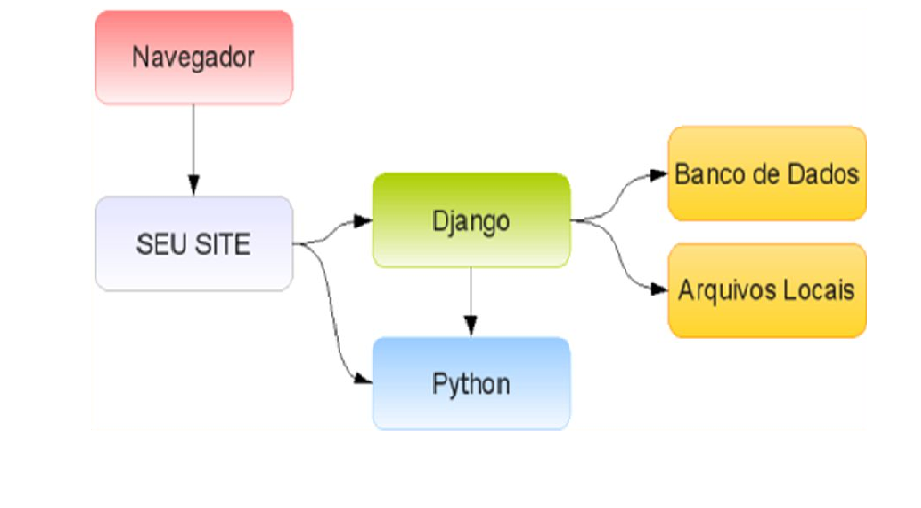
\includegraphics[width=20em]{figuras/arquiteturadjaongo.png}}
   
    \centerline{Fonte : www.slideplayer.com.br/django}
\end{figure}


\section{JSON}
JSON é um formato de dados Javascript Object Notation (Notação de Objetos Javascript)
para ser mais exato ele é derivado dos objetos literais da linguagem de programação Javascript,
Isso faz do JSON um subconjunto da linguagem Javascript.Embora seja um subconjunto da linguagem
de programação o JSON não é uma linguagem de programação, mas sim um formato para trocas de dados. JSON pode ser definido também como uma representação textual por um pequeno conjunto de  regras segundo o qual os dados são estruturados \cite{smith2015beginning}. O formato de arquivo JSON,será utilizado como formato de dados para trabalhar com as requisições para as APIs. No exemplo da figura 4.1  logo abaixo, pode se ver como e o formato de dados  JSON. 

\begin{figure}  [h]
    \caption{ Exemplo de formato JSON}
    \centerline{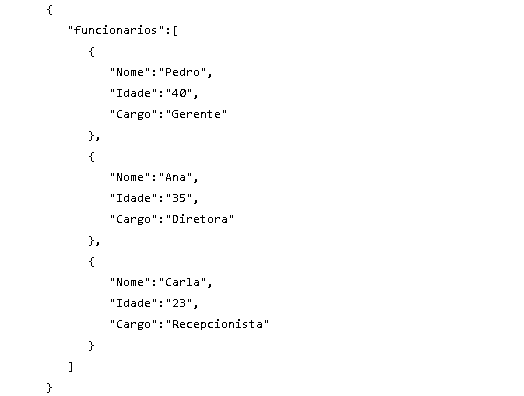
\includegraphics[width=20em]{figuras/img4.png}}
    \centerline{Fonte :www.matera.com}
\end{figure}

\section{API}

API é um conjunto de rotinas e padrões de programação para acesso a um aplicativo de \textit{software}. Um exemplo de API pode ser visto como um cliente fazendo um pedido de recurso para um servidor.O pedido é tecnicamente chamado de requisição. O pedido é feito à API do servidor solicitado. A API recebe essa requisição e consulta o serviço responsável por organizar a chegada das requisições e buscar os recursos requisitados. O servidor então processa a requisição e retorna o que foi solicitado ou retorna uma exceção caso não encontre  ou ocorra algum erro na solicitação que foi pedida \cite{saudate2014rest}.


\section{API de Reconhecimento Visual IBM Watson}

O reconhecimento visual usa algoritmos de aprendizagem profunda para analisar imagens que podem dar-lhe informações sobre o seu conteúdo visual.A API  permite organizar bibliotecas de imagens, analisar uma imagem individual, reconhecer alimentos, detectar rostos e criar classificadores personalizados para resultados específicos adaptados às necessidades \cite{APIVISUAL}.

O serviço de reconhecimento visual da IBM, oferece uma API, no padrão cliente servidor onde e possível através dessa API, realizar cadastro de classificadores personalizados, este projeto fará uso dessa API para o desenvolvimento do aplicativo.




\chapter{Levantamento de Requisitos}
O levantamento de requisitos consiste em entender as necessidades do sistema perante
seu usuário final, bem como separar os requisitos por necessidade e por dois tipos:
funcionais e não-funcionais.

Os requisitos funcionais correspondem à definição de funcionalidades gerais e principais
do sistema, enquanto os requisitos não funcionais se referem às restrições, condições
e validações que devem ser consideradas perante os requisitos funcionais previstos (Guedes,2011). Os requisitos abaixo foram baseados em diversos trabalhos semelhantes.



\section{Requisitos Funcionais}


\begin{table}[h]
\caption{Requisitos Funcionais}
\begin{center}
\begin{tabular}{|l|l|l|}
\hline RF001 &  Cadastrar Usuário  &  O sistema deve permitir o \\  & & cadastro de usuários.\\
\hline RF002 &  Listar Usuários  & O sistema deve permitir listar usuários.\\
\hline RF003 &  Autenticar Usuário  & O sistema deve permitir autenticação.\\
\hline RF004 &  Alterar Perfil  & O sistema deve permitir alterar dados \\  & & cadastrados do usuário.\\
\hline RF005 & Diagnosticar Doença de Pele  & O sistema deve tentar analisar a  \\  & & imagem enviada para análise.\\


\hline 
\end{tabular}
\centerline{Fonte: autor}
\end{center}
\end{table}    



\section{Requisitos Não-Funcionais}
   Os requisitos não-funcionais do sistema estão listados na Tabela 5.2.

\begin{table} [h]
\caption{Requisitos Não Funcionais}
\begin{center}
\begin{tabular}{|l|l|}
\hline RN001 &  O sistema deve estar disponível 50\% do dia para acesso.\\
\hline RN002 &  O sistema deve ser capaz de suportar múltiplas plataformas   \\
\hline RN003 &  Adaptar-se as resoluções igual ou abaixo de 1140 x 900px \\ 
 & ou igual ou acima de 320 x 568px   \\
\hline 
\end{tabular}
\centerline{Fonte: autor}
\end{center}
\end{table}    
    
    \vspace{2cm}
    
\section{Modelagem do Sistema}

\subsection{Arquitetura do Sistema}

Para o padrão de projeto, será adotado o padrão de projeto Modelo, Visão e Controlador (MVC), cujo padrão de arquitetura de software visa separar a lógica de negócio da lógica de apresentação, permitindo o desenvolvimento, teste e manutenção isolado de ambos. O modelo é usado para definir e gerenciar o domínio da informação e notificar observadores sobre mudanças nos dados. A visão apresenta o modelo num formato adequado ao utilizador, na saída de dados, e diferentes visões podem existir para um mesmo modelo, para diferentes propósitos.
O controlador recebe a entrada de dados e inicia a resposta ao utilizador ao invocar objetos do modelo, e por fim uma visão baseada na entrada. Ele também é responsável pela validação e filtragem da entrada de dados \cite{silveira2012introduccao}.

\begin{figure}  [h]
\caption{Arquitetura MVC}
    \centerline{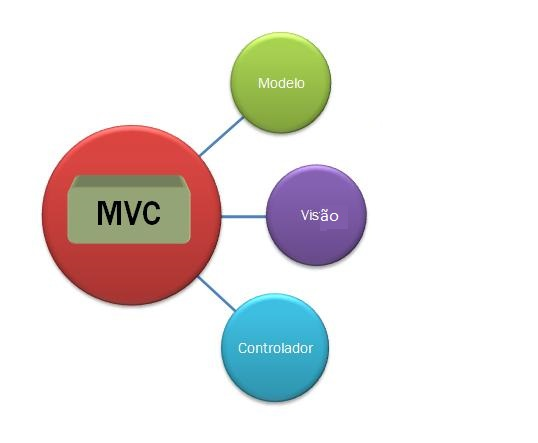
\includegraphics[width=30em]{figuras/mvc_architectural_pattern.jpg}}
    
    \centerline{Fonte : www.commons.wikimedia.org}
    \label{mvc}
\end{figure}

\begin{itemize}
  \item  Modelo - É considerado o componente central da aplicação e expressa o comportamento da mesma na questão de solucionar o problema gerado pela ação do usuário, independentemente da interface do usuário. Gerencia o comportamento e os dados e responde a pedidos de informação (geralmente vindos da View) e a instruções de mudança de estado (geralmente por parte do Controller).

\item Visão - Essa parte é responsável pela resposta gráfica e/ou textual da ação iniciada pelo usuário.

\item Controlador - É a parte que interpreta as ações do usuário (feitas pelo mouse ou teclado) e se comunica com a View, manipulando informações extraídas do Model de acordo com o resultado pretendido.

\end{itemize}


\subsection{Diagrama ER}
O Modelo Entidade Relacionamento (também chamado Modelo ER) é um modelo de dados conceitual de alto nível, bastante usado na fase de planejamento de um software, geralmente após a análise de requisitos. O Modelo ER é um modelo de dados conceitual bastante popular e usado para representar o comportamento das tabelas (entidades) do banco de dados e suas relações umas com as outras \cite{elmasri2015fundamentals}.

Abaixo se encontra o Diagrama ER da solução proposta, que conta com 4 tabelas:

A entidade \textbf{users} armazena os dados dos usuários do sistema. Os dados dessa tabela são populados na tela de cadastro de usuários. Essa tabela é composta por quatro colunas obrigatórias, sendo elas id, name, email e password, sendo as outras colunas opcionais para esta tabela. É através dessa tabela que o sistema valida a autenticação do usuário para logar no sistema.


A tabela \textbf{classifiers} armazena os dados dos classificadores criados no sistema, foi adicionado essa tabela pois o sistema vai utilizar mais de um classificador. Os dados de tabela são armazenados cada vez que o usuário administrador cria um classificador dentro do sistema. É através dessa tabela que o software mantem relação com os classificadores que foram criados na API do IBM Watson, e essa tabela possui 4 colunas obrigatórias sendo elas  id,name, ident,status e uma coluna opcional chamada description. A entidade \textbf{class} é responsável por armazenar as classes de cada classificador criado no sistema. Essa tabela possui todas colunas obrigatórias, e essa entidade mantém relacionamento com a tabela classifiers onde o relacionamento indica que para cada classe existe um classifier. 



\begin{figure}  [h]
    \centerline{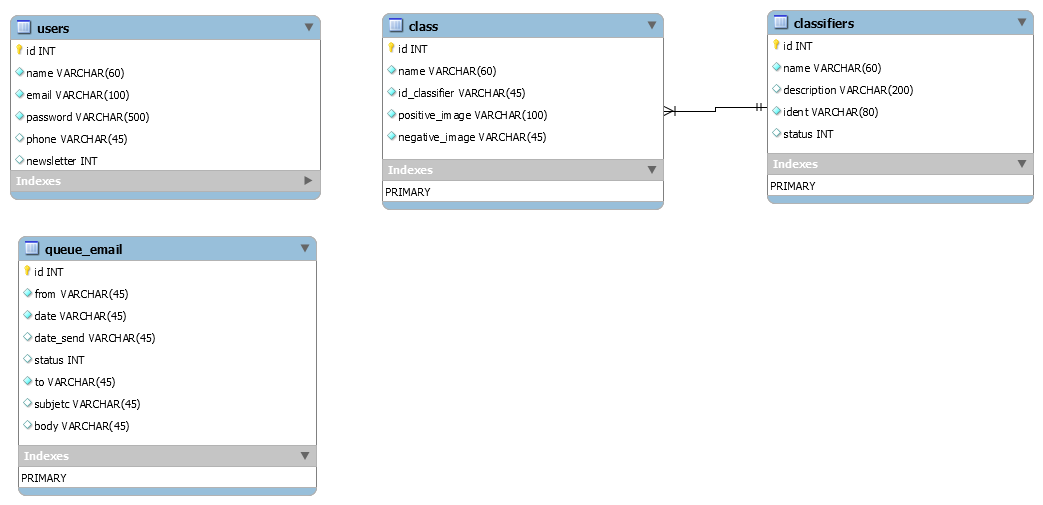
\includegraphics[width=35em]{figuras/ER.png}}
    \caption{Diagrama ER}
    \centerline{Fonte:autor}
\end{figure}


 Finalmente, a tabela \textbf{queue\_email}  que é responsável por armazenar as mensagens enviadas via e-mail entre os usuários e o sistema. Essa entidade serve como uma fila de mensagens que o sistema armazena para ter um controle do que está sendo enviado e do que já foi enviado para os usuários. Ela possui quatro colunas obrigatórias, sendo elas: id, from, to, date e quatro colunas opcionais. 




\subsection{Diagrama de  Casos de Uso}

O diagrama de caso de uso é elaborado geralmente na fase de levantamento de requisitos do sistema e serve de base para desenvolvimento dos demais diagramas necessários para representação de um projeto \cite{guedes2008uml}.

Abaixo o diagrama de caso de uso dos usuários do Skin System, representando as ações possíveis dentro do sistema que podem ser realizadas pelos usuários, como representado na imagem da Figura (Figura:\ref{caseuso}). 
Este diagrama foi baseado na representação contida na obra de Guedes (2011, p.98).

\textbf{Realizar Login} -  Essa é a parte na qual o usuário se autentica no sistema com e-mail e senha sendo requisitados ao usuário.


\textbf{Gerenciar Perfil} - O usuário poderá atualizar seus dados cadastros dentro do aplicativo. Para realizar essa ação o usuário deve estar logado no sistema.


\textbf{Diagnosticar Doenças} -Esta ação representa a principal funcionalidade do aplicativo: nela o usuário vai adicionar a foto no aplicativo e vai submeter à análise do sistema, o sistema vai consultar a API do IBM Watson, através do identificador dos classificadores.

\textbf{Gerenciar Classificadores} - Essa área  do aplicativo é destinada ao ator admistrador; é nessa parte que são criados os classificadores, juntamente com suas classes. O sistema nessa versão terá apenas um classificador de doenças.

\textbf{Visualizar Lista de Usuários} - Essa ação do software será para o administrador visualizar os usuários que se cadastraram, servindo como um relatório para o ator. 

\textbf{Criar Conta no Sistema} - Nessa parte o usuário paciente realizará o cadastro no aplicativo. Essa ação consiste no usuário preencher os dados do formulário de cadastro e submeter ao sistema; com isto, caso os dados estejam válidos, o sistema criará a conta do usuário que solicitou.



\begin{figure}  [h]
    \centerline{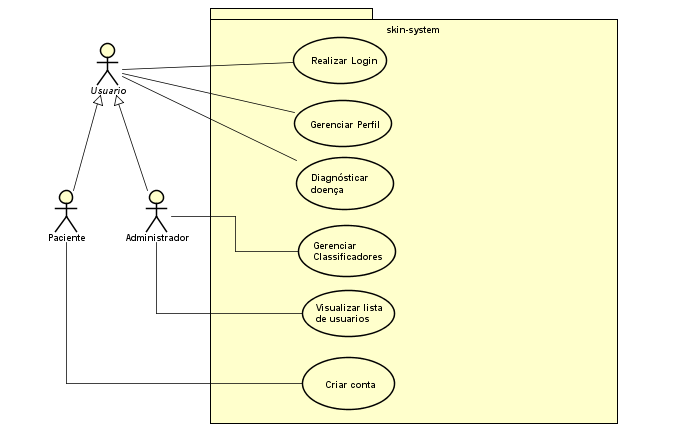
\includegraphics[width=30em]{figuras/casodeuso.png}}
    \caption{ Diagrama de Caso de uso},
    \label{caseuso}
    \centerline{Fonte:autor}
\end{figure}

\subsection{Diagrama de Atividades}
O diagrama de atividades se preocupa em descrever os passos a serem realizados para conclusão de uma atividade especificada, podendo esta ser representada por um método com certo grau de complexidade, um algoritmo, ou mesmo por um processo completo.
O Diagrama de atividade concentra-se na representação do fluxo de controle de uma atividade ou processo \cite{guedes2008uml}.


A imagem abaixo (Figura: \ref{atividadeim}) apresenta os passos sequenciais utilizados para a realização do 
diagnóstico. Os primeiros passos são realizados pelo usuário, onde o mesmo é responsável por  se autenticar no sistema, posicionar o dispositivo de forma que a imagem capturada da lesão atenda a condição de estar contida totalmente dentro do espaço da imagem. Caso a imagem adquirida não atenda a essa condição, o usuário pode repetir essa operação repetidas vezes, até que o mesmo obtenha uma imagem aceitável para a condição imposta pelo sistema. Após a aquisição da imagem, o usuário submete a mesma ao processamento do sistema e a partir
desse ponto o sistema se encarrega de efetuar todos os passos necessários para analisar a lesão.

\begin{figure}  [ht]
\caption{Diagrama de atividade}
    \centerline{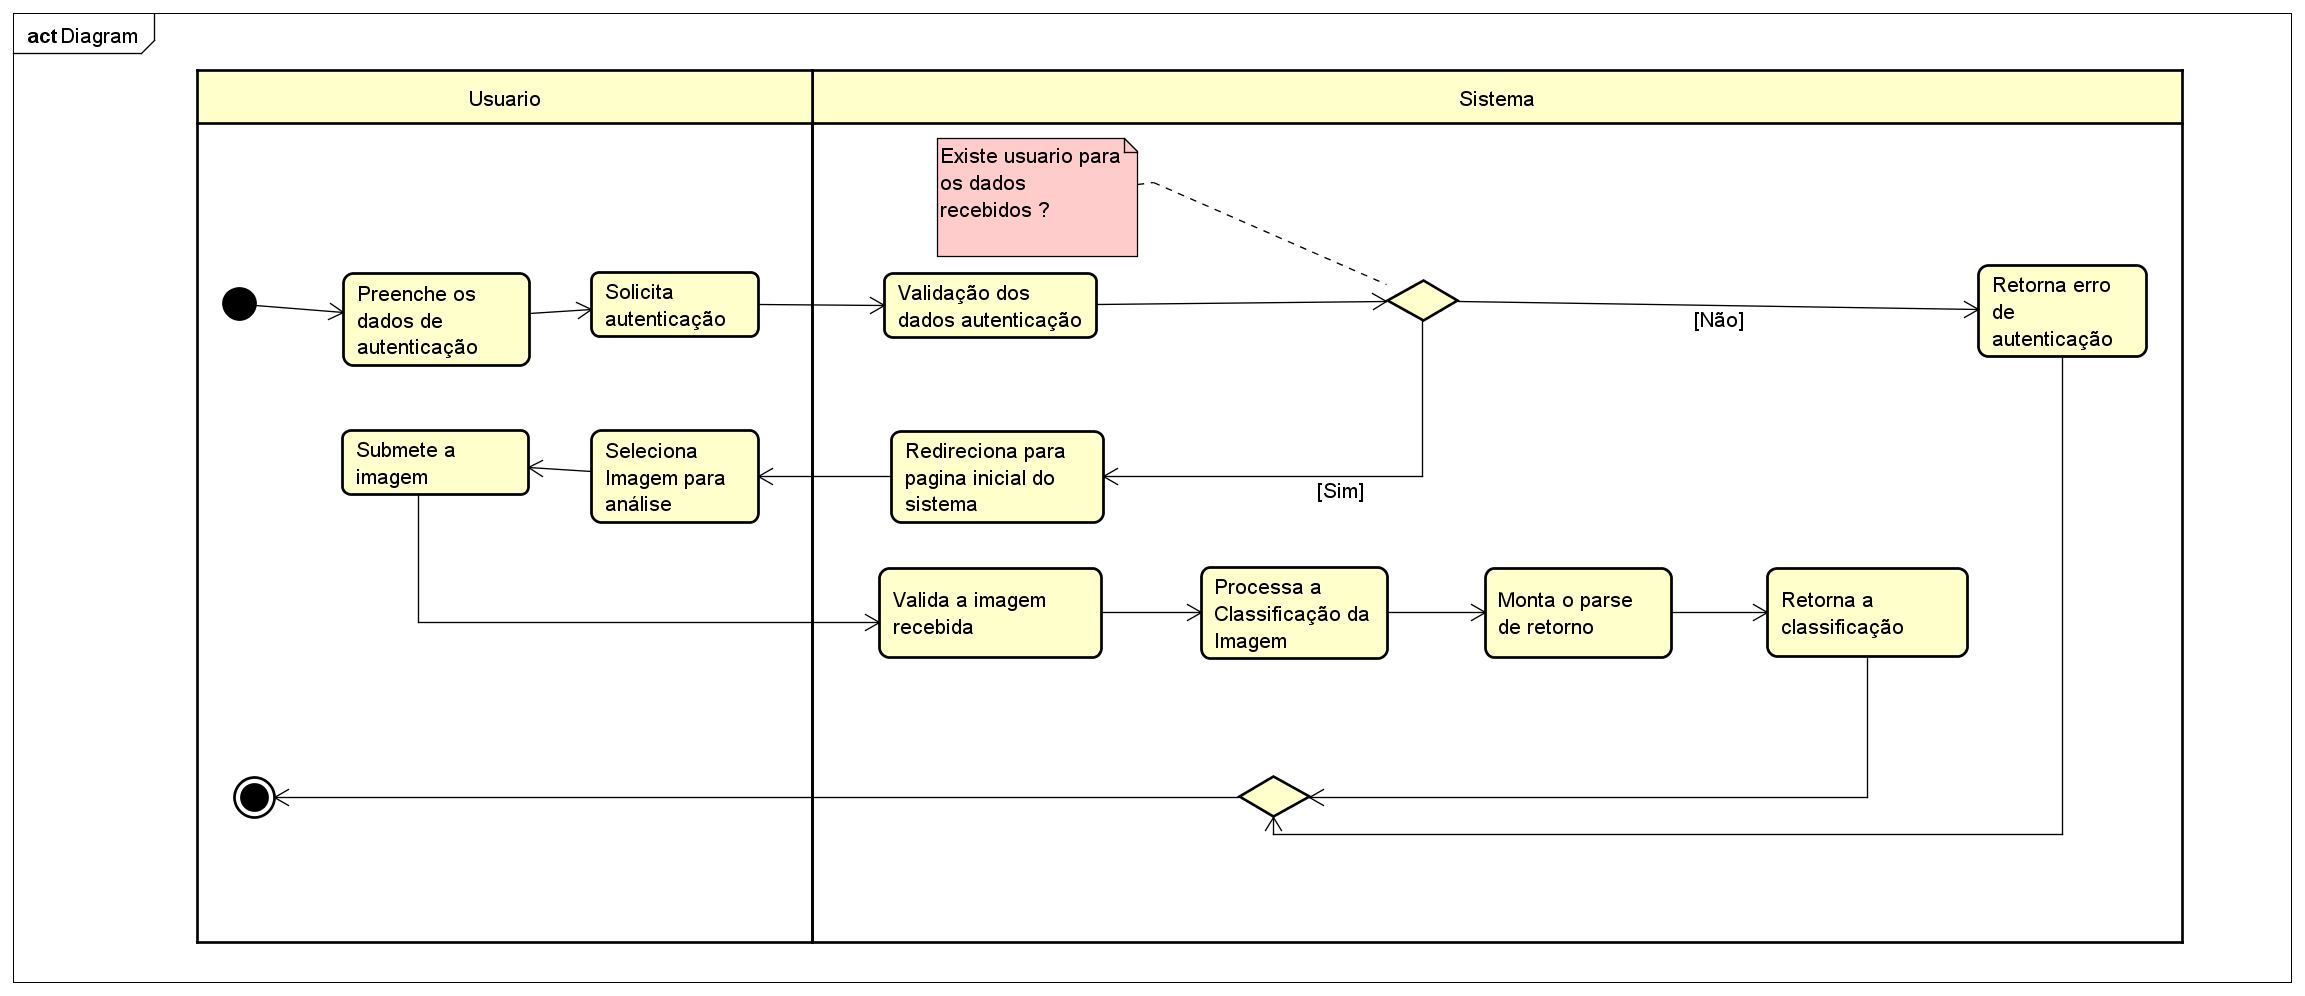
\includegraphics[width=40em]{figuras/atividade.png}}
    
    \label{atividadeim}
    \centerline{Fonte:autor}
\end{figure}

\subsection{Diagrama de Classes}
O diagrama de classes tem como objetivo esclarecer os métodos e atributos das classes
do sistema, e como estas se relacionam entre si. É outro diagrama que serve para fundamentar
o sistema e é usado como base para a criação de outros diagramas. O diagrama de classes representa o sistema com uma visão estática de como as classes estão organizadas, tendo como responsabilidade aclarar a estrutura lógica das mesmas (Guedes, 2011).

A representação das classes do aplicativo em questão é apresentado na Figura \ref{diagramaclasscompl}, presente no apêndice A. Na figura \ref{parcialclass} há  outro diagrama  contendo apenas as principais classes do sistema.
Nota-se pelo padrão MVC que as classes se comunicam em camadas, mas a única camada que tem classes comunicantes entre si é a de Model, que no caso cria os tipos principais de objetos do sistema (isto é, possui os atributos principais).


A camada de visão não está no diagrama por conta de esta ser representada por saídas
nos próprios códigos de interface (em geral HTML com trechos da comunicação controladora
e View em Python). A camada modelo do sistema contém a estrutura-base das classes do sistema, bem como os principais métodos para enviar e receber informações no banco de dados. A camada controladora recebe todas as requisições feitas pela parte do cliente, encaminhando o retorno solicitado ou código do erro caso ocorra um erro. Juntamente com o modelo MVC, utilizou-se uma outra estrutura de pacote chamada de Service (Serviço), onde é realizada a maioria das regras do sistema, e ela fornece uma centralização nas regras de negócio.

Abaixo estão descritas as classes da camada controladora: 


A classe \textbf{LoginController} é responsável por realizar a autenticação no aplicativo, possui  os métodos  \textbf{do\_login}, responsável por receber os dados de autenticação do formulário HTML, o método \textbf{register} que é responsável pelo cadastro do usuário, o método \textbf{resetPass} que possibilita o usuário substituir sua senha caso tenha perdido, e por fim o método \textbf{do\_logout} que realiza a saída do usuário no sistema, limpando a sessão do navegador e redirecionando para fora do sistema.  


A classe \textbf{UserController} é responsável por listar e atualizar os dados do usuário logado. Ela apresenta os métodos \textbf{index}, \textbf{update} e \textbf{save}.



A classe \textbf{HomeController} tem por objetivo somente mostrar a página inicial do sistema, retornando o conteúdo HTML da mesma. Ela apresenta o método \textbf{index}. 


A classe \textbf{ErrorController} é responsável por tratar dos erros que podem vir a ocorrer no sistema como, por exemplo, um erro de página não encontrada. Essa classe possui o método \textbf{page\_not\_found} e o atributo statusCode que será atribuído ao status de retorno caso haja um erro.



A classe \textbf{ClassifierController} é a classe principal do sistema, pois a principal funcionalidade do sistema se encontra nela e é responsável pela criação do classificadores pelo administrador. Nela também é realizada a classificação da imagem submetida pelo usuário. A classe possui os métodos  \textbf{index}, \textbf{add}, \textbf{getDisease}, \textbf{removeClassifier}, \textbf{getAllClassifiers}.



Abaixo estão descritas as classes da camada de modelo e do pacote FormModel:

%-------------------------------------------------


A classe \textbf{Classifier} contém os atributos necessários para ser criado um classificador no banco de dados, e enviado para API de reconhecimento visual do IBM Watson.


A classe \textbf{Class} contém os atributos de uma classe de um classificador, como os atributos nome, descrição e id. Essa classe se relaciona com a classe de classificadores, sendo esta uma relação de composição forte, pois um classificador não existe sem uma  \textbf{Class}.


A classe \textbf{User} é responsável pelos dados do usuário. Ela apresenta os atributos que contém um usuário como name, email, password, phone e newsletter.



A classe \textbf{FormUser} é responsável por persistir e buscar os dados do usuário e abstrair métodos de validação de dados de formulário HTML.


A classe \textbf{FormClassifier} é responsável por persistir e buscar os dados do classificador e abstrair uns métodos de validação de dados de formulário HTML.


Abaixo estão descritas as classes do pacote serviço (service):

A classe \textbf{Upload} é responsável por tratar do upload de arquivos do sistema, possuindo o  \textbf{setDir}, que especifica o diretório do sistema operacional onde serão guardados os dados recebidos, e um método process que realiza a transferência dos dados.



A classe \textbf{Watson} é responsável por abstrair todos os métodos disponíveis na API de reconhecimento de Imagens IBM Watson e é nessa classe que fica a comunicação entre o sistema proposto e API onde fica o classificador utilizado. Ela possui os métodos \textbf{createClassifier}, \textbf{deleteClassifier}, \textbf{classifier}, \textbf{listClassifiers}, 
\textbf{updateClassifier} e \textbf{prepareRequest}.


A classe \textbf{LayoutPaginator} é responsável por realizar a paginação dinâmica  dos resultados buscados no banco de dados. É através dessa classe que o sistema apresenta as tabelas no  HTML  com limite de resultados por página .

A classe \textbf{Image} tem como objetivo o processamento de Imagens no sistema e possui o método \textbf{processImages}, que realiza o processamento das imagens recebidas pelo \textbf{Upload}. O processamento realizado e o de rotação, translação e escala nas imagens recebidas, assim gerando outras combinações de imagens.


Abaixo, na Figura, está o diagrama de classes com as principais classes.


\begin{figure}  [h]
  \caption{ Diagrama parcial de classes}
    \centerline{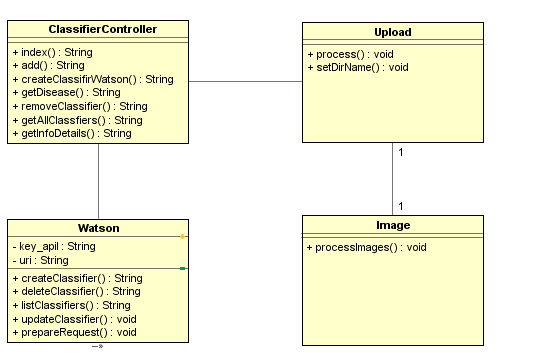
\includegraphics[width=30em]{figuras/parte_classe.png}}
  
    \label{parcialclass}
    \centerline{Fonte:autor}
\end{figure}



\chapter{Desenvolvimento}
Este capítulo pretende explicar o aplicativo web Skin System de maneira funcional. São apresentadas explicações e capturas de tela com as interações que o usuário terá com a interface do Skin System. As funcionalidades principais são abordadas e a explicação das tecnologias utilizadas para o desenvolvimento das mesmas será descrita.

\section{Login}

Os dados para validação do login são compostos pelo e-mail e senha do usuário. Caso não haja um login válido ou seja a primeira utilização, o cadastro pode ser
feito através de link presente na mesma página. O cadastro pede informações básicas como nome, e-mail, senha e repetição da mesma, como apresentado na imagem (Figura: \ref{cadlog}) abaixo:

\begin{figure}  [h]
   \caption{Tela  cadastro e login }
    \centerline{
       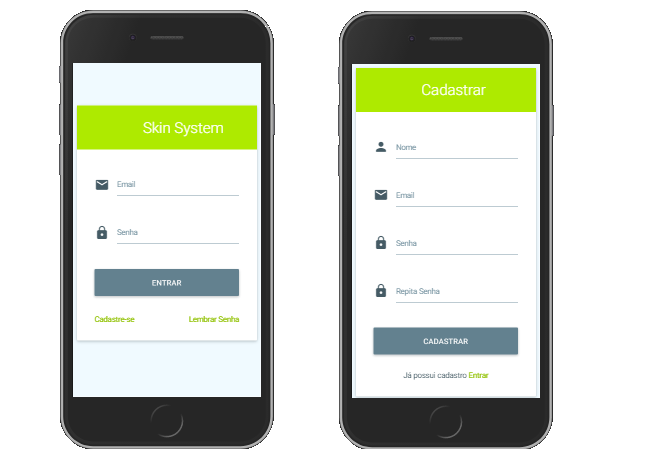
\includegraphics[width=30em]{figuras/sistema/login_cadastro_phone.png}
     }
   
    \label{cadlog}
    \centerline{Fonte:autor}
\end{figure}

Existe  validação no formato de e-mail e comparação das duas senhas, mostrando alerta caso elas não sejam a mesma. O aplicativo também oferece  na tela de login  a opção de alterar a senha caso o usuário tenha esquecido  a sua senha.


A aplicação realiza a busca dos dados inseridos no banco de dados da aplicação. A conectividade é feita por conta da interface de conexão do Django. As validações desse processo envolvem checagem de modelo de e-mail (deve conter um "@"e um ponto final na url após o "@") e exibição de erro caso algum dos dois dados de autenticação estejam incorretos.

Para validar o acesso, é executado o código da figura (Figura:\ref{authlo}) a seguir. Nesse trecho o sistema recebe a requisição como parâmetro no método e então  repassa para  o método \textbf{authenticate}, que está dentro do \textit{framework} Django. Este método retorna uma instância de usuário. Caso essa instância não esteja vazia, o sistema permite a entrada do usuário. Caso contrário, ele recebe um alerta na tela.


\begin{figure}  [h]
   \caption{Trecho de código do login}
    \centerline{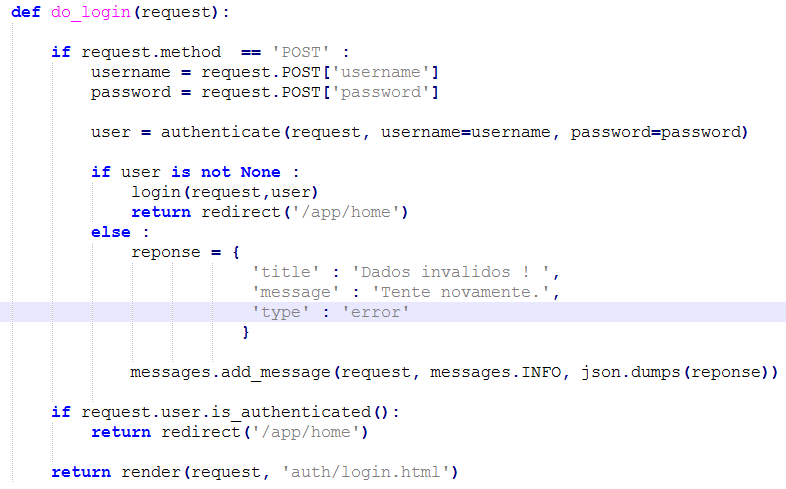
\includegraphics[width=1.0\textwidth]{figuras/login_codigo.png}}
  
    \label{authlo}
    \centerline{Fonte:autor}
\end{figure}

\section{Diagnóstico da Doença}
Essa é a principal tela, pois é nela que o usuário paciente vai submeter uma imagem para
ser analisada pela ferramenta. Nessa tela o usuário arrasta ou clica na área  de upload da arquivo. Depois que o usuário seleciona a imagem, ele clica no botão com lupa,
como esta na imagem abaixo (Figura: \ref{diagnosticimg}).

\begin{figure}  [h]
   \caption{Tela de análise de imagem}
    \centerline{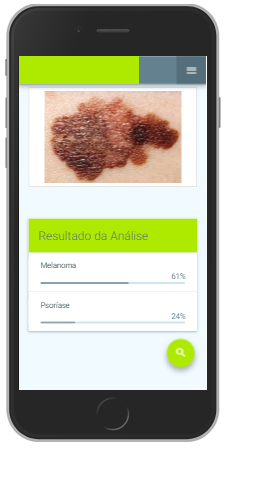
\includegraphics[width=0.5\textwidth]{figuras/diagnostico_ima.png}}
    \label{diagnosticimg}
    \centerline{Fonte:autor}
\end{figure}

O sistema apresenta se conseguiu ou não realizar a análise. Caso tenha conseguido, ele vai mostrar uma 
tabela com o nome das doenças cadastradas e uma barra de porcentagem mostrando a chance de ser a doença. Essa requisição é feita pelo navegador através da linguagem javascript. Depois de receber o retorno, o próprio javascript monta o HTML da tabela e injeta o resultado na página.
Esses dados retornados do sistema e apresentados ao paciente são os dados que o classificador da API de Reconhecimento Visual  da IBM retorna. Este Retorno é um JSON 
contendo o nome do classificador, uma lista das classes e o valor da confiança para cada classe. Esse valor de confiança retornado vai de 0 a 1.
Para solicitar essa análise ao classificador, o sistema faz uma requisição com o protocolo 
HTTP através da classe service para a API do Watson. Na figura abaixo (Figura : \ref{codesvcimg}) temos um exemplo de código da classe service que faz essa requisição.

\begin{figure}  [h]
 \caption{Trecho de código da requisição à API}
    \centerline{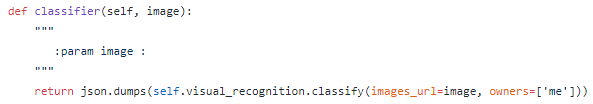
\includegraphics[width=0.8\textwidth]{figuras/codesvcimg.png}}
    \centerline{Fonte: autor}
    \label{codesvcimg}
\end{figure}



Depois de processar a requisição, a classe service recebe um JSON similar ao mostrado na próxima imagem (Figura: \ref{diagnosticjson}) e então a classe faz  
formatação do retorno, retornando para o cliente (navegador) que fez a solicitação.



\begin{figure}  [h]
    \caption{JSON retornado da API para classificação de imagem}
    \centerline{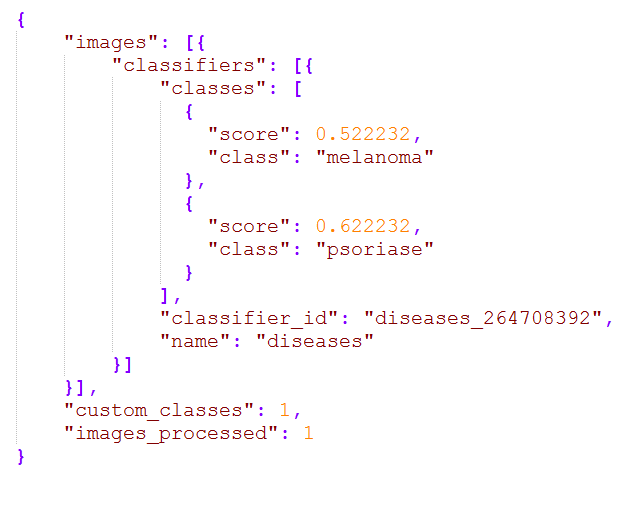
\includegraphics[width=0.5\textwidth]{figuras/ret_class_json.png}}

    \label{diagnosticjson}
    \centerline{Fonte: autor}
\end{figure}

\clearpage


\section{Perfil}
No perfil do usuário, o usuário poderá  atualizar alguns dados do seu cadastro. Nessa tela o sistema apresenta  três abas, sendo uma \textbf{Perfil}, onde o usuário poderá  alterar campos como nome, telefone e e-mail. Na aba de \textbf{Senha} se pode alterar a mesma preenchendo ambos campos disponíves com a nova sequência de caracteres a ser utilizada para entrada no sistema. A outra aba é a de \textbf{Notificações} e serve para  que o usuário possa
definir as suas configurações de privacidades, ou seja, o que ele quer receber do sistema ou não. A figura a seguir (Figura : \ref{profileimg}) exemplifica a interface citada.

\begin{figure}  [h]
 \caption{Tela perfil usuário}
    \centerline{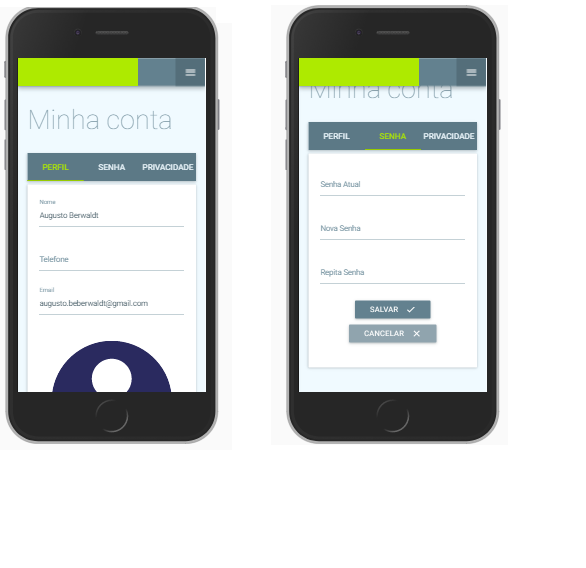
\includegraphics[width=30em]{figuras/sistema/perfil.png}}
   
    \label{profileimg})
    \centerline{Fonte: autor}
\end{figure}



\section{Listagem de Usuários}


Ao realizar o login com usuário administrador, o aplicativo lista no menu lateral a opção
 \textbf{Usuários}, onde o administrador pode visualizar os usuários cadastrados até o momento.
 Essa tela serve como um relatório e futuramente poderá ter mais opções nessa área como, por exemplo, editar ou desativar usuários cadastrados no sistema. Nessa tela, o sistema busca todos usuários cadastrados na tabela de users para realizar essa consulta.
 A imagem abaixo (Figura: \ref{lisadmuser}) apresenta tela de listagem de usuários.

\begin{figure} [h]
 \caption{Tela listagem de Usuários}
    \centerline{
    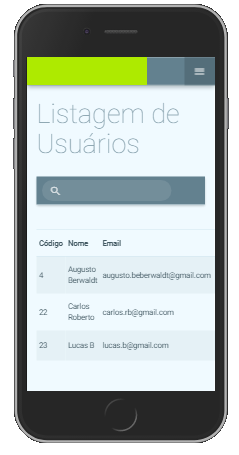
\includegraphics[width=15em]{figuras/sistema/listagem_usuarios_phone.png} }
   
    \label{lisadmuser}
    \centerline{Fonte: autor}
\end{figure}


\clearpage
\subsection{Cadastro de Classificador}

Nessa área do aplicativo será possível visualizar e criar classificadores. Somente o usuário administrador possui acesso a essa parte da aplicação. Para criar  um classificador o sistema pede alguns dados, conforme representado na imagem abaixo (Figura : \ref{classifierimg})


\begin{figure}  [h]
 \caption{Tela de cadastro de classificador}
    \centerline{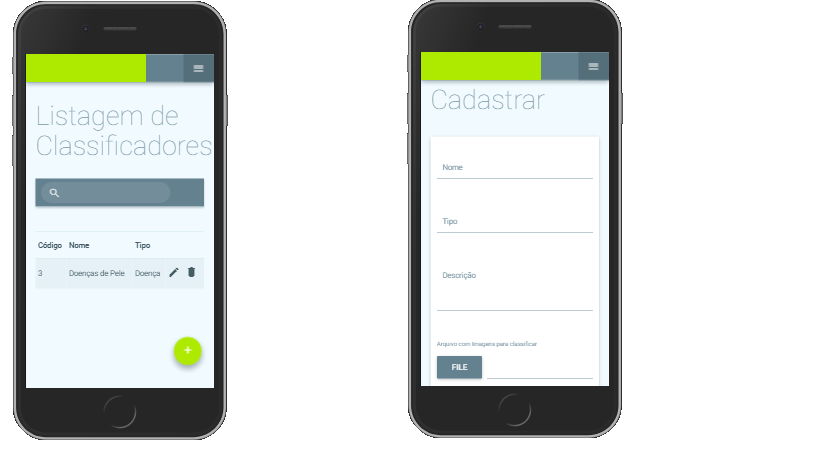
\includegraphics[width=30em]{figuras/sistema/cadastro_lista_class.png}}
   
    \label{classifierimg}
    \centerline{Fonte:autor}
\end{figure}

Para realizar esse cadastro, tanto no banco de dados do sistema como na API do IBM Watson, o sistema recebe os dados vindos do formulário HTML,
processa as informações recebidas e persiste no banco  MYSQL. Depois de persistir os dados, o sistema envia uma requisição HTTP através da classe Watson. Após enviar solicitação HTTP, o sistema recebe o  retorno da API, que retorna JSON, conforme pode ser visto na imagem a seguir (Figura : \ref{classifierretjson}).

\begin{figure} [h]
  \caption{Retorno da API}
    \centerline{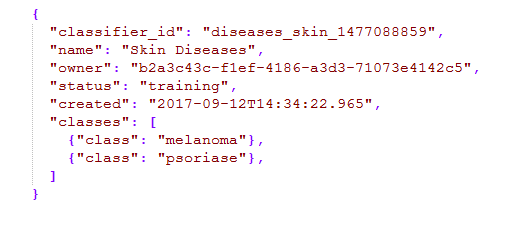
\includegraphics[width=30em]{figuras/json_ibm.png}}
  
    \label{classifierretjson}
    \centerline{Fonte:autor}
\end{figure}

Depois de criado o classificador, a API demora alguns minutos para treinar o mesmo. Depois de o treinar, realizamos a consulta na API para verificar o status do classificador e ver se ele já está pronto para ser usado. Caso esteja pronto, ele retorna status \textbf{ready}. 

\clearpage

\section{Testes e Resultados}
Para  realizar o treinamento, foram utilizadas  as imagens da base DermNet NZ \cite{dermnetnzsite}, que fornece imagens catalogadas por nome de doença.
Também foram utilizadas algumas imagens do site da Sociedade Brasileira de Dermatologia \cite{SBC}.

Para analisar os resultados, foi observado o valor de confiança retornado do classificador para um número  de 320 imagens, 10 imagens da doença melanoma e mais 10 de psoríase, onde foi utilizado o \textit{data augmentation} para aumentar o teste e ficar com total 320 imagens,através desses valores foi montado  a  matriz de confusão. A matriz de confusão é a forma de representação da qualidade obtida de uma classificação digital, sendo expressa por meio da correlação de informações dos dados de referência (compreendido como verdadeiro) com os dados classificados. Essa rotina também pode ser expressa pela análise das amostras de treinamento juntamente com os dados classificados.


Abaixo segue a representação das matrizes de confusão obtidas através dos testes.

\begin{table}[h]
\centering
\caption{Matriz de Confusão da doença de Melanoma}

\label{mconfusao}

\begin{tabular}{lllll}
\cline{1-4}
\multicolumn{2}{|l|}{\multirow{2}{*}{}}                                                & \multicolumn{2}{l|}{Classe Real}                              &  \\ \cline{3-4}
\multicolumn{2}{|l|}{}                                                                 & \multicolumn{1}{l|}{Negativo} & \multicolumn{1}{l|}{Positivo} &  \\ \cline{1-4}
\multicolumn{1}{|l|}{\multirow{2}{*}{Classe Prevista}} & \multicolumn{1}{l|}{Negativo} & \multicolumn{1}{l|}{64}        & \multicolumn{1}{l|}{60}        &  \\ \cline{2-4}
\multicolumn{1}{|l|}{}                                 & \multicolumn{1}{l|}{Positivo} & \multicolumn{1}{l|}{38}        & \multicolumn{1}{l|}{104}        &  \\ \cline{1-4}
                                                       &                               &                               &                               &  \\
                                                       &                               &                               &                               & 
\end{tabular}
\centerline{Fonte:autor}
\end{table}


\begin{table}[h]
\centering
\caption{Matriz de Confusão da doença de Psoríase}

\label{mconfusao}

\begin{tabular}{lllll}
\cline{1-4}
\multicolumn{2}{|l|}{\multirow{2}{*}{}}                                                & \multicolumn{2}{l|}{Classe Real}                              &  \\ \cline{3-4}
\multicolumn{2}{|l|}{}                                                                 & \multicolumn{1}{l|}{Negativo} & \multicolumn{1}{l|}{Positivo} &  \\ \cline{1-4}
\multicolumn{1}{|l|}{\multirow{2}{*}{Classe Prevista}} & \multicolumn{1}{l|}{Negativo} & \multicolumn{1}{l|}{104}        & \multicolumn{1}{l|}{18}        &  \\ \cline{2-4}
\multicolumn{1}{|l|}{}                                 & \multicolumn{1}{l|}{Positivo} & \multicolumn{1}{l|}{36}        & \multicolumn{1}{l|}{64}        &  \\ \cline{1-4}
                                                       &                               &                               &                               &  \\
                                                       &                               &                               &                               & 
\end{tabular}
\centerline{Fonte:autor}
\end{table}



A matriz utiliza  uma tabela (com duas linhas e duas colunas) que relata o número de falsos positivos (FP), falsos negativos (FN),  verdadeiros positivos (VP) e verdadeiros negativos (VN). Podemos observar na tabela Tabela: \ref{mconfusao} que na posição (x1, y1) encontra-se o VP,  na posição (x1, y2) encontra-se o FP, na posição (x2, y1) encontra-se FN, e por sua vez na posição (x2,y2) encontra-se o VN. 

Foi utilizado essa matriz pois para cada  doença foi criado um classificador informando a classe com  as imagens das doenças e uma classe negativa (imagens do que não é classe criada), essa classe e obrigatória para criação do classificador na API, pois como cada classificador é um classificador binário onde o classificador compara uma classe contra todas as outras, no caso do sistema Skin system ele vai comparar somente uma classe com a classe negativa ou seja com as imagens do que não é a doença. O retorno é sempre o valor de uma classe (não  retorna o valor das outras classe, pois a classificação é binária), por isso foi criado um classificador para cada doença. Onde o classificador compara a classe da doença com a classe negativa enviada. Cada classificador sempre retorna um valor independente de ser uma doença ou não.

Como visto nas tabelas, o sistema classificou das 160 imagens  104 sendo da doença de melanoma. Nas 160 imagens refentes a psoríase o sistema classificou 64 como sendo doença de psoríase. Todas as previsões corretas estão localizadas na diagonal principal da tabela. Com essa tabela , podemos perceber também que o classificador pode vir a classificar errado uma doença como por exemplo no caso onde o sistema avaliou que 96 imagens de psoríase sendo como  nenhuma por isso e considerado um falso negativo (FN).


Com os dados da matriz de confusão foi realizado o cálculo da acurácia. Para se calcular o valor de acurácia  pode se  utilizar as seguintes equações:

\[ACURACIA = NUMERO\_DE\_ACERTOS / TOTAL\_DE\_TESTES\]

\[ACURACIA =   (VP + VN) / (POSITIVAS + NEGATIVAS) \]

O banco de imagens foi formado por 50 imagens de melanoma e mais 50 de psoríase, onde as imagens  passaram por um algoritimo de modificação de escala, translação e rotação, com essa combinação foram geradas diferentes imagens para uma mesma imagem. Os valores alterados para escala foram de 
0.5, 2 e para translação -100, +100 e por fim a rotação dos ângulos foi  de  90$^{\circ}$, 180$^{\circ}$, 270$^{\circ}$, 360$^{\circ}$. Com essa combinação, temos para cada imagem mais 16, se pegarmos  nossa amostra de 100 imagens e multiplicarmos teremos um
total de 1600 imagens compondo a base do classificador, essa ténica foi mencionada anterirormente como sendo \textit{data augmentation}.


\begin{figure}  [h]
 \caption{Exemplo do  \textit{data augmentation} aplicado nas imagens das doenças }
    \centerline{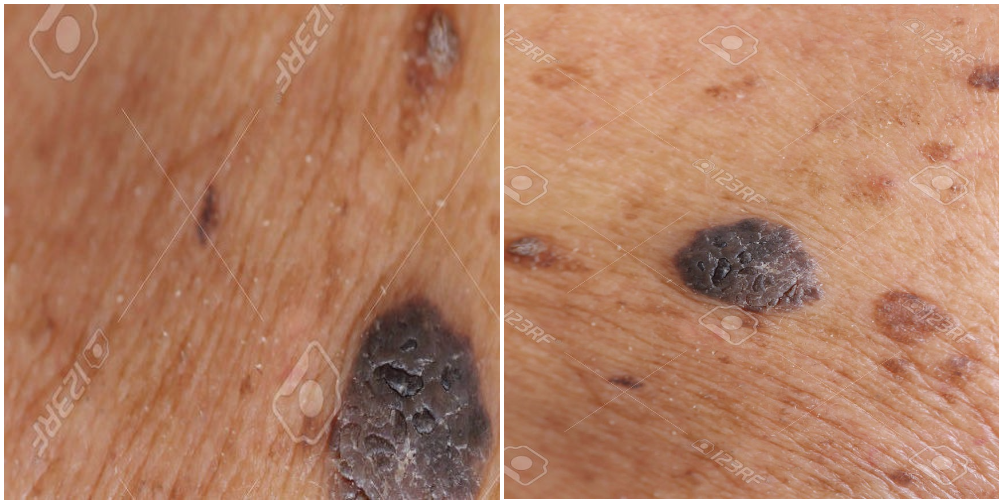
\includegraphics[width=20em]{figuras/data_aug_melanoma.png}}
     \centerline{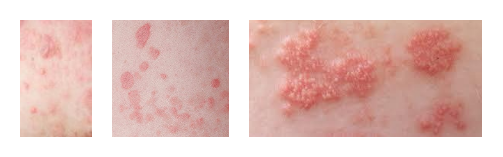
\includegraphics[width=30em]{figuras/data_augementation.png}}
    \label{classifierimg}
    \centerline{Fonte:autor}
\end{figure}

\vspace{2cm}



Para o resultado final da classificação, foram realizados 8 ciclos no treinamento, sendo a validação realizada com o teste de maior acurácia, que foi de 53\%. Nos outros treinamentos realizados, houve problemas na técnica de   \textit{data augmentation} , onde foi utilizado ângulos impares para rotação das iamgens, fazendo com que alguns cantos das imagens ficassem preto. outro problema enfrentado foi a a amostragem de imagens, no inicio dos teste sem a utilização da técnica \textit{data augmentation} o valor da  acurácia era maior, por ter uma amostragem peguena. Com a ampliação dos dados utilizando o  \textit{data augmentation},  o valor da acurácia foi diminuindo, pois o classificador tem mais dados para analisar. O valor de  acurácia será apresentado no sistema, como  é um valor fixo ele aparecera fixo no sistema para o usuário.

 O código-fonte da  aplicação esta  disponível 
 no Github. O Github é um repositorio online de fontes. Para acessar o código do projeto  basta acessar a url : \url{https://github.com/augustoberwaldt/skin-system}.


\chapter{Conclusão}

Neste trabalho foi apresentado o desenvolvimento de um sistema de classificação de imagens dermatoscópicas para plataforma web, sendo adaptável para dispositivos móveis, utilizando o serviço de reconhecimento visual do IBM watson. O objetivo desse sistema é fornecer uma ferramenta que possa auxiliar pacientes ou  profissionais de saúde na análise de doenças de pele através de um aplicativo web. O uso do sistema deve possibilitar e facilitar o acesso ao exame de dermatoscopia nas regiões mais interioranas, na zona rural e nas regiões onde não existe a presença de especialistas. Uma outra aplicação para esse sistema é facilitar o processo de triagem de pacientes, além de possibilitar a formação de uma base de imagens que pode ser utilizada para o acompanhamento do paciente, para possíveis estudos sobre dermatoscopia e para testes com outras técnicas para análise de lesões de pele.

Como trabalhos futuros, sugere-se o uso de um conjunto com uma maior quantidade de imagens dermatoscópicas, pois um conjunto de dados maior pode vir a melhorar o desempenho do classificador. Também analisar a viabilidade do desenvolvimento de um classificador próprio, e não utilizar uma API de terceiros. Outro ponto seria tamem ter mais doenças cadastradas para abrangir
mais o escopo de doenças de pele.

Seria também interessante expandir o sistema quanto à gerência dos dados adquiridos, onde o usuário possa organizar e melhorar o acesso aos dados, adicionando a possibilidade do usuário salvar o histórico das análises. Outro fator a ser considerado é a busca de parcerias com especialistas e/ou hospitais com o objetivo de adquirir imagens e validar as funções do sistema.






% carrega o arquivo com as bibliografias e põe o capítulo com as referências neste lugar
\bibliography{bibliografia}



\appendix

\chapter{Diagrama de Classes Completo}
\begin{figure}  [h]
    \centerline{
        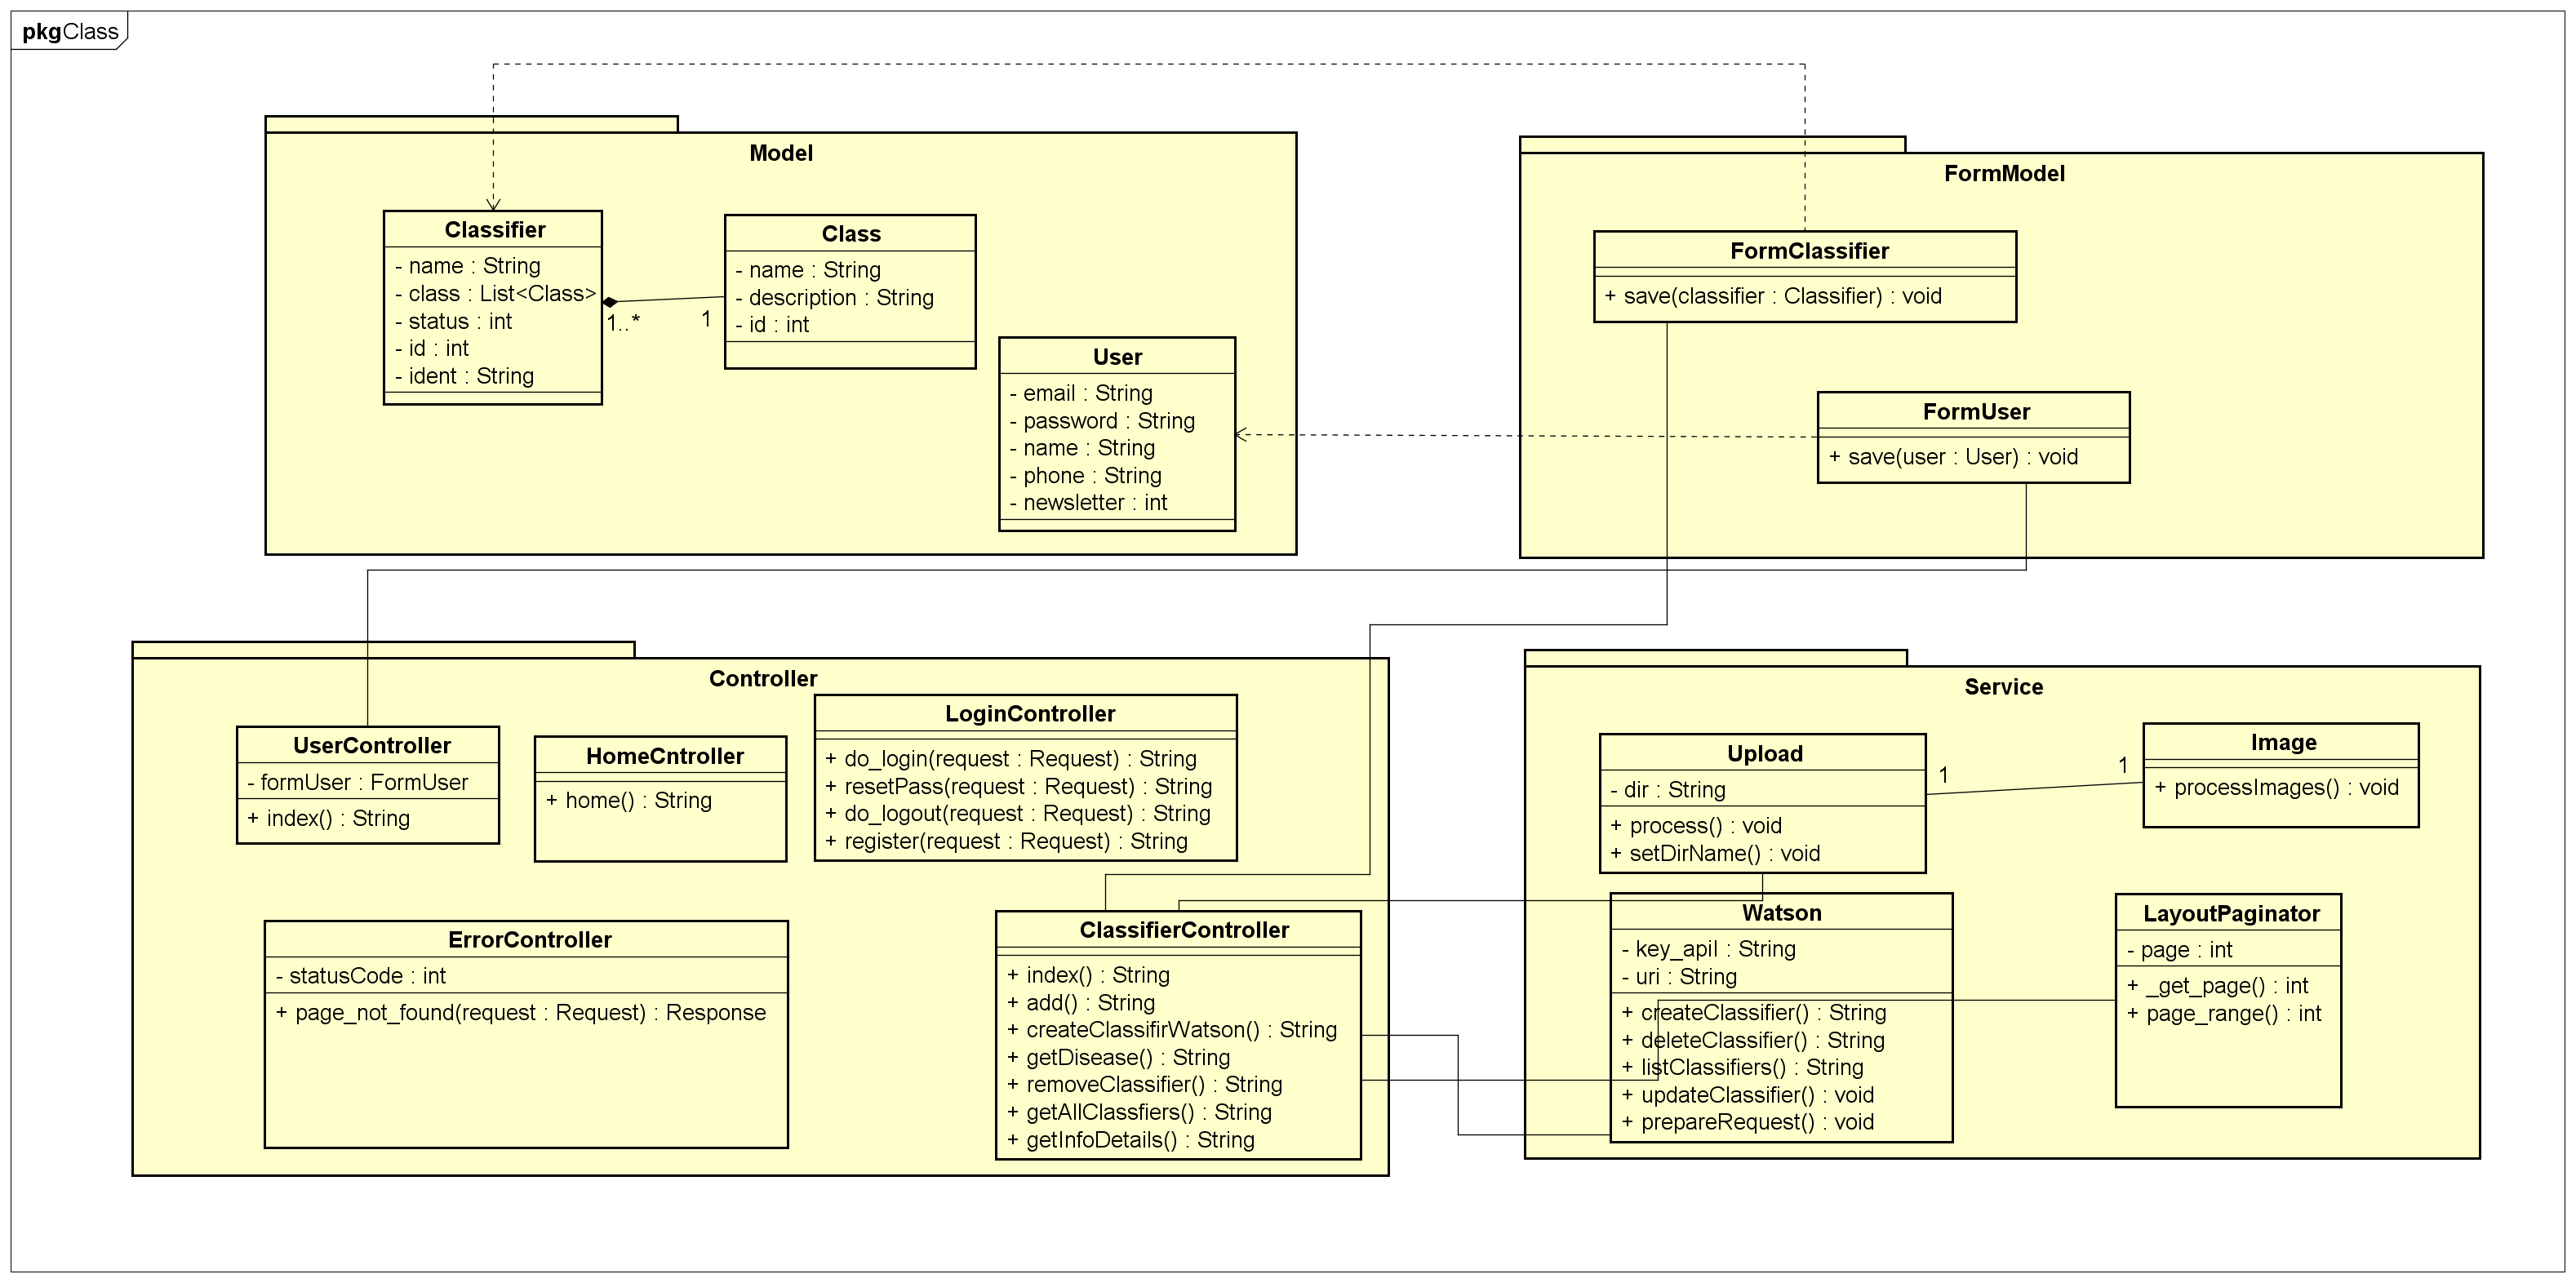
\includegraphics[width=40em,angle=90]
        {figuras/sistema/diagramadeclasses.png}
    }
    \caption{ Diagrama de Classes}
    \label{diagramaclasscompl}
    \centerline{Fonte:autor}
\end{figure}


% a partir daqui, todo capítulo novo é apêndice
%\appendix

%\chapter{Anexos e Apêndices}
%Destinam-se à inclusão de informações complementares ao trabalho, mas que não são essenciais à sua compreensão. Os Apêndices devem apresentar material desenvolvido pelo próprio autor, formatado de acordo com as normas. Já os Anexos destinam-se à inclusão de material como cópias de artigos, manuais, etc., que não necessariamente precisam estar em conformidade com o modelo, e que não foram desenvolvidos pelo autor do trabalho.

%importa dicasLatexABNT.tex para o Apêndice 
%\input{dicasLatexABNT.tex}

\end{document}







 
